\documentclass{beamer}
\usepackage[utf8]{inputenc}
\usepackage[]{amsmath}
\usepackage{graphicx}
\usepackage{subcaption} % package pour faire des subfigures
\usepackage{multirow} % package pour multirow/multicolumn
\usepackage{booktabs} % package pour top/mid/bottom rule
\usepackage{tcolorbox} % toujours plus de boites
\usepackage[backend=biber]{biblatex}


\addbibresource{Biblio_dbl_quantum.bib}

%\bibliographystyle{stylename}
%\bibliography{Biblio_dbl_quantum}

\title{Mechanical and relaxation-based detection of dipolar-interactions between spins in diamond}
\author{Clément Pellet-Mary\\ Laboratoire de physique de l'ENS\\ \textit{ENS, Paris}}
\date\today

\mode<presentation> {\usetheme{Rochester}}

\begin{document}
\begin{frame}
\maketitle
\end{frame}
\begin{frame}{Two experiments around cross-relaxations in diamond}
\includegraphics[scale=.3]{Shémas_intro}
\end{frame}
\begin{frame}{Outline}
\tableofcontents
\end{frame}
\section{Nitrogen Vacancy center presentation}
\begin{frame}{Outline}
\tableofcontents[currentsection]
\end{frame}
\begin{frame}{Minimalist approach to NV center}
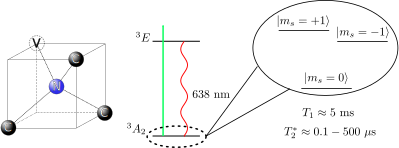
\includegraphics[scale=.28]{NV_prez_generale}
\end{frame}
\begin{frame}{Triplet spin levels at rest}
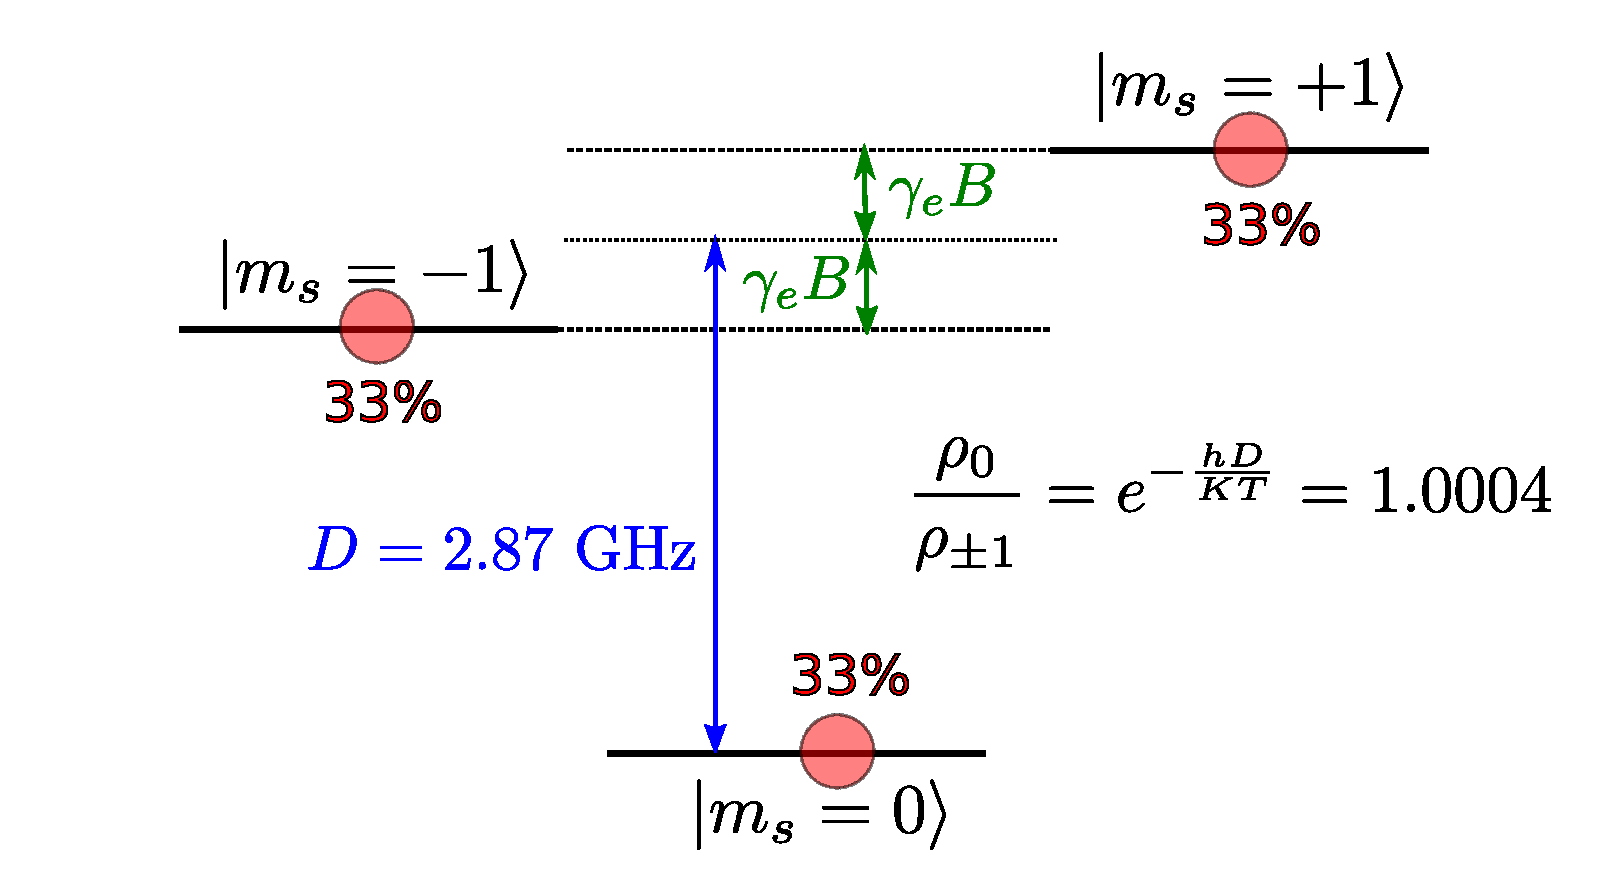
\includegraphics[scale=.4]{3_niveaux_1}
\end{frame}
\begin{frame}{Triplet spin levels with optical pumping}
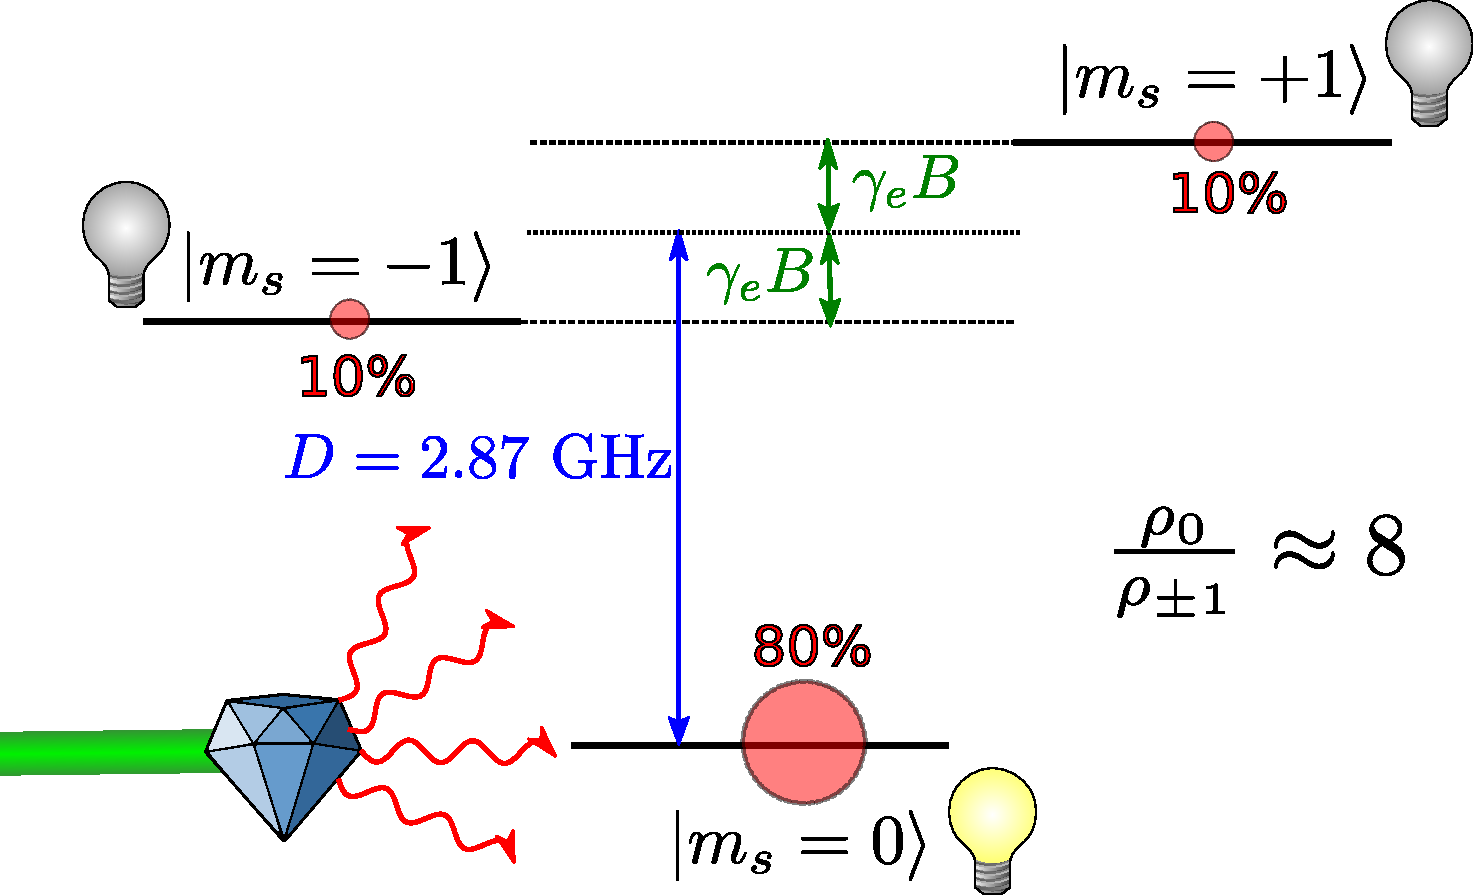
\includegraphics[scale=.4]{3_niveaux_2}
\end{frame}
\begin{frame}{Magnetometry with NV centers : ODMR with a single spin}%"Efficient population transfer"
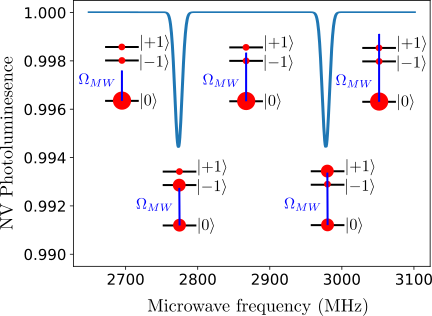
\includegraphics[scale=.65]{ESR_1spin_simu}
\end{frame}
\begin{frame}{Spin Hamiltonian and orientation of the centers}
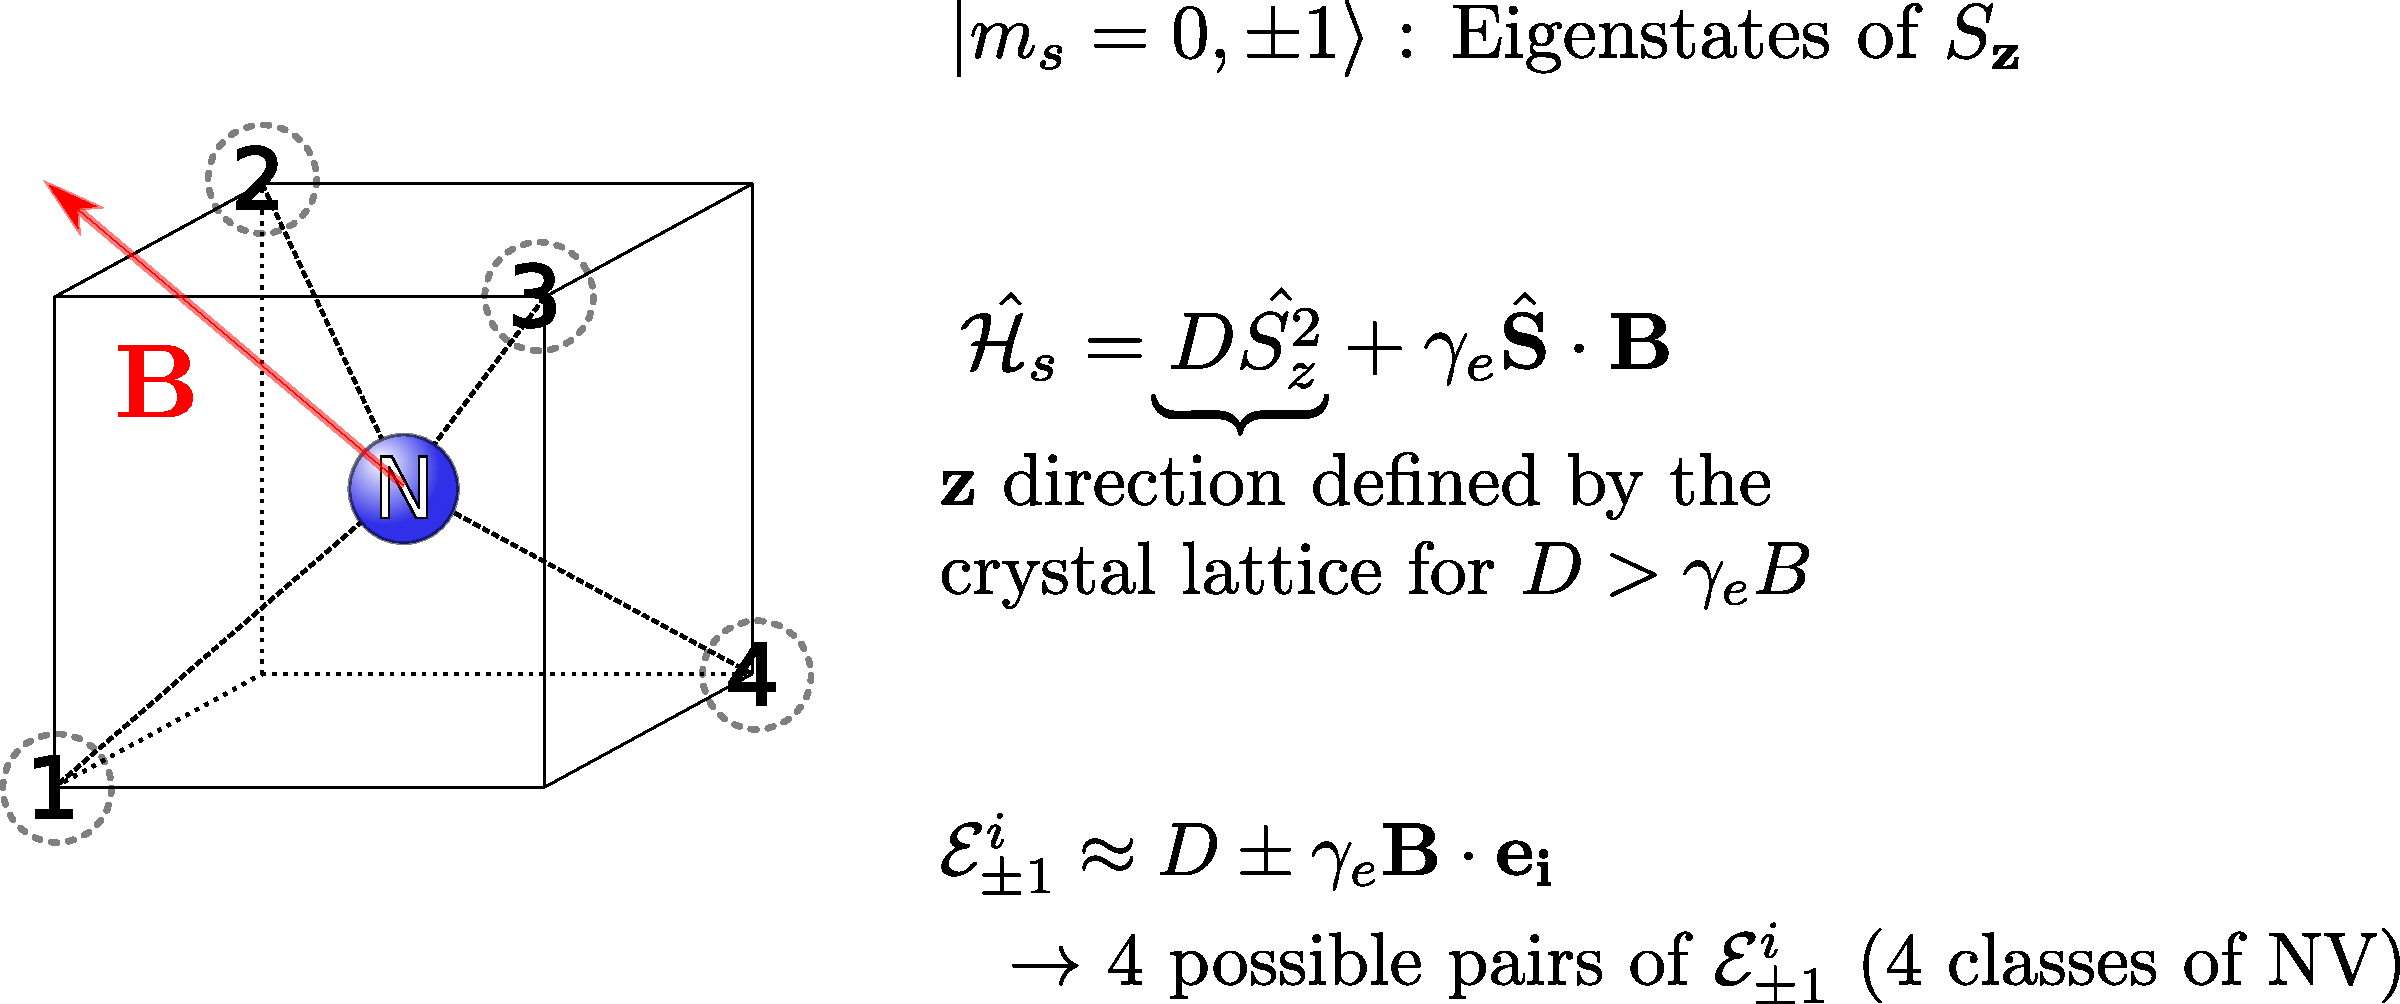
\includegraphics[scale=.25]{projection_4_classes}
\end{frame}
\begin{frame}{ODMR with an ensemble of NV centers}
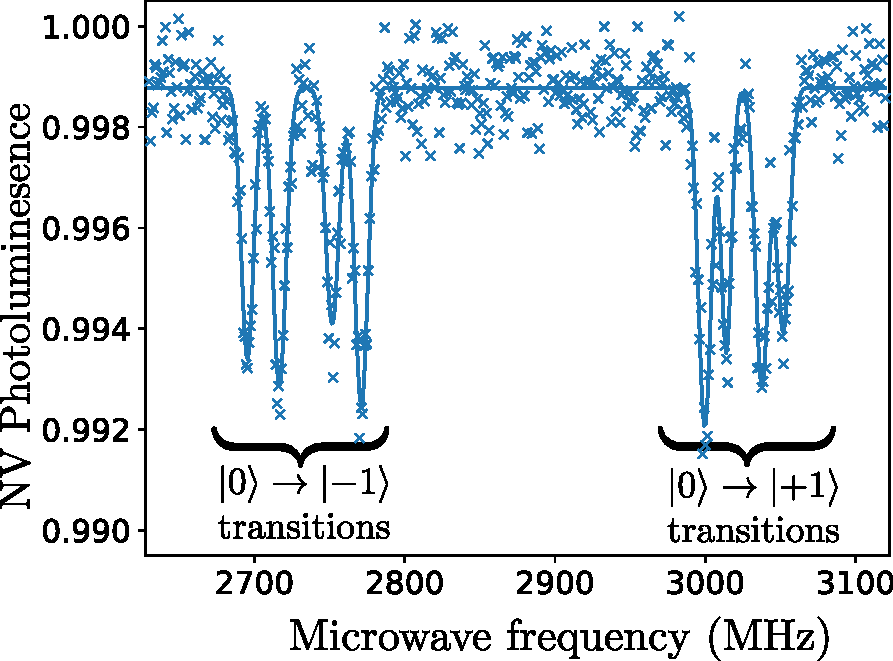
\includegraphics[scale=.65]{ESR_4spin_simu}
\end{frame}
\section{Cross-relaxations with new spin species}
\begin{frame}{Outline}
\tableofcontents[currentsection]
\end{frame}
\begin{frame}{Photoluminescence change with magnetic field amplitude}
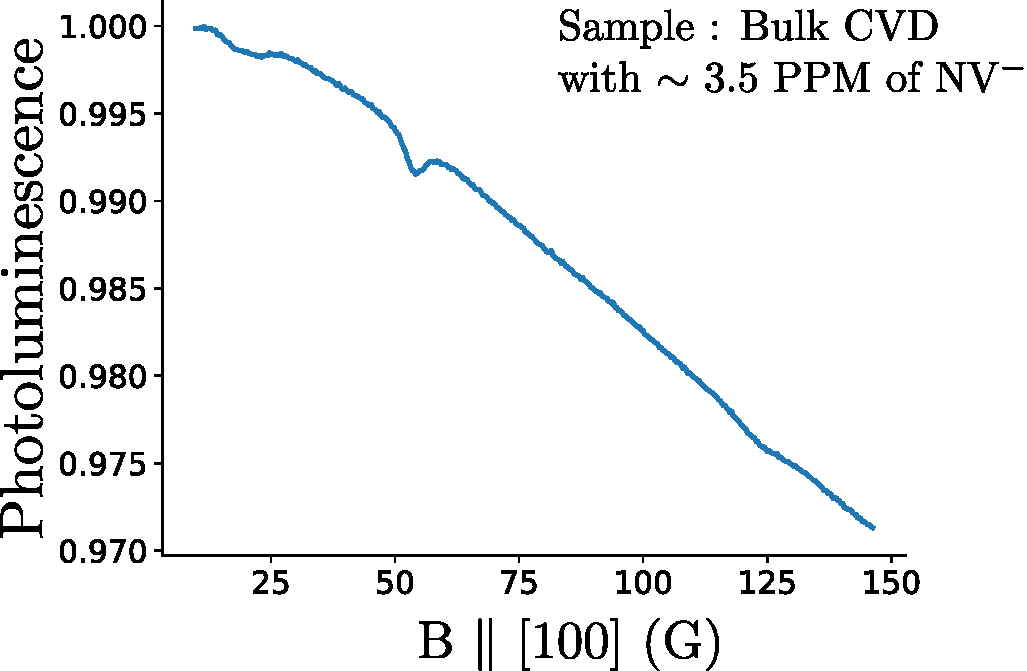
\includegraphics[scale=.62]{Scan_100_0}
\end{frame}
\begin{frame}{PL change with magnetic field : [100] direction}% "Cubic cell"
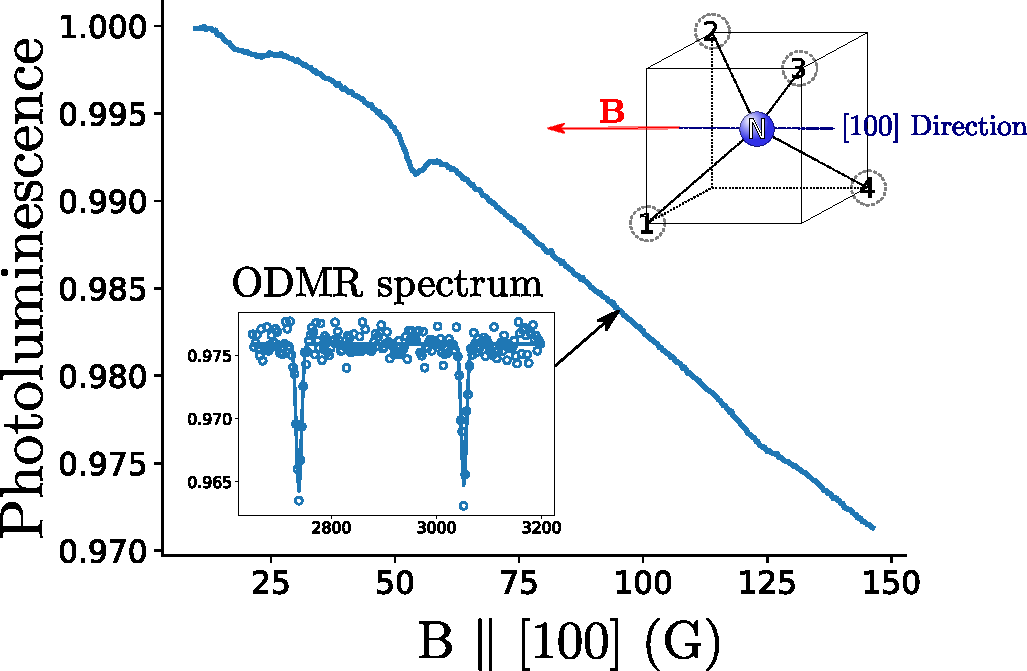
\includegraphics[scale=.62]{Scan_100_1}
\end{frame}
\begin{frame}{PL change with magnetic field : transverse field}
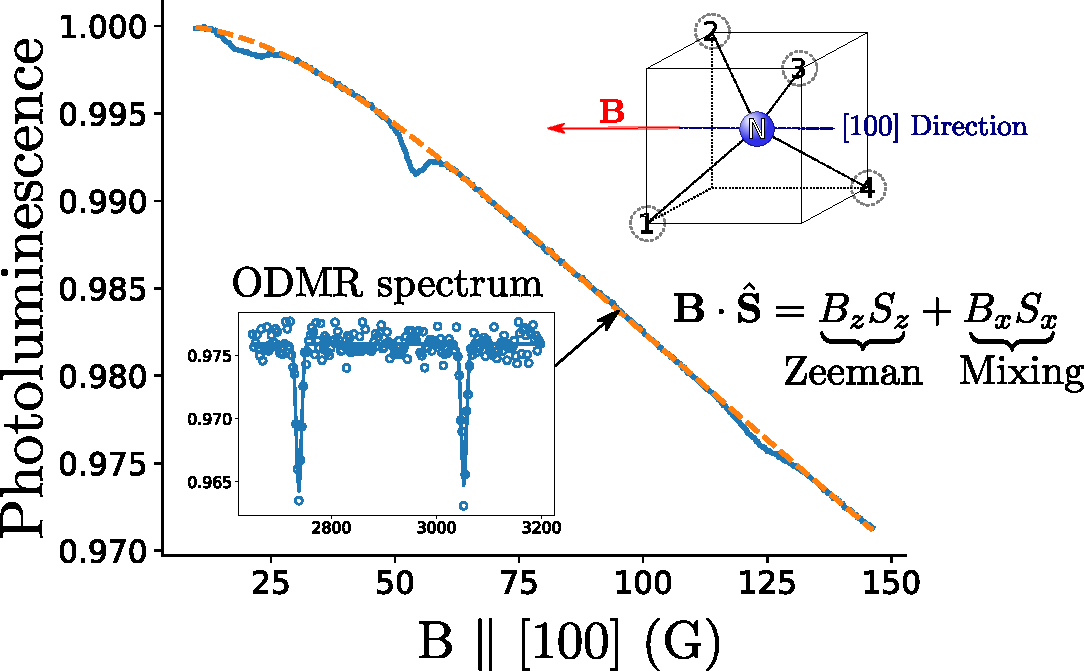
\includegraphics[scale=.62]{Scan_100_2}
\end{frame}
\begin{frame}{Subtracting the transverse field envelope}
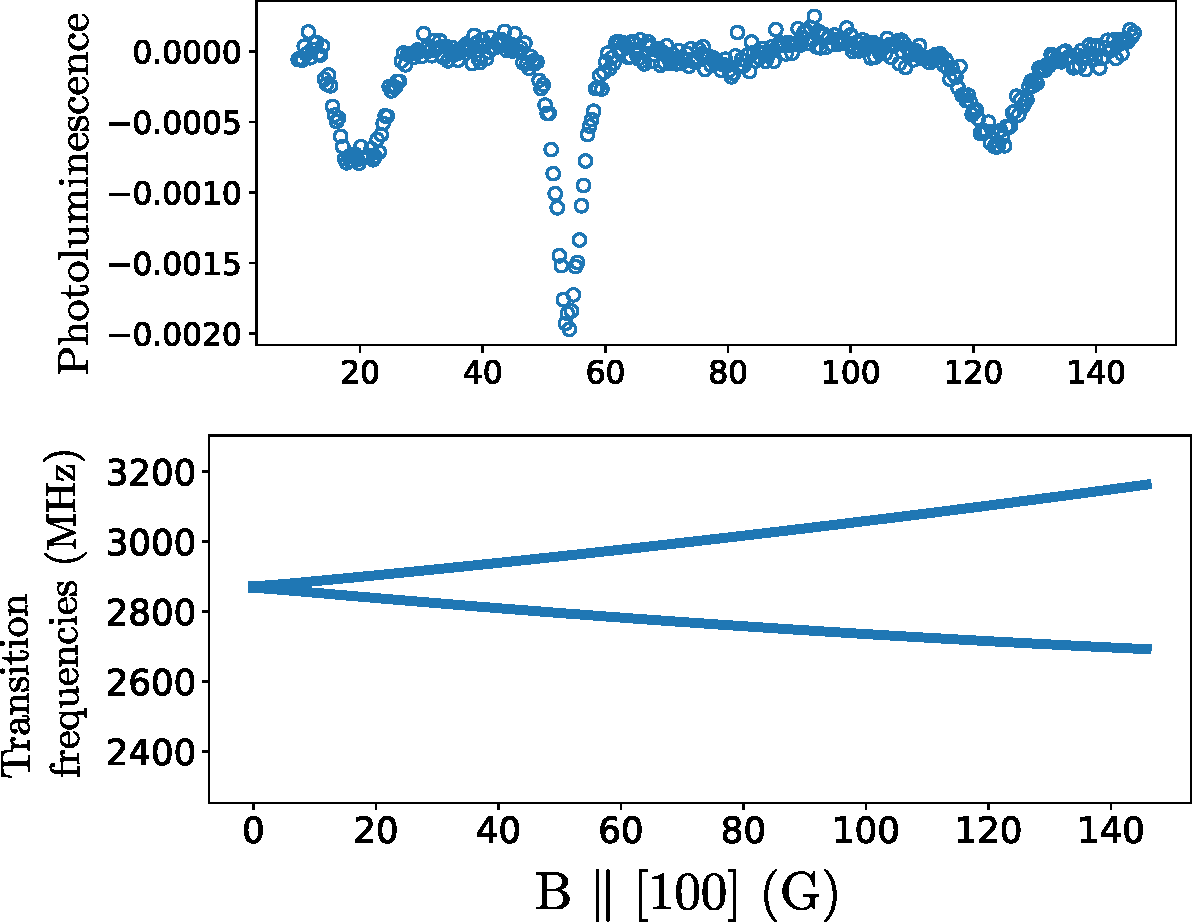
\includegraphics[scale=.48]{soustraction_0}
\end{frame}
\begin{frame}{Cross-relaxation between NV$^-$ and VH$^-$}
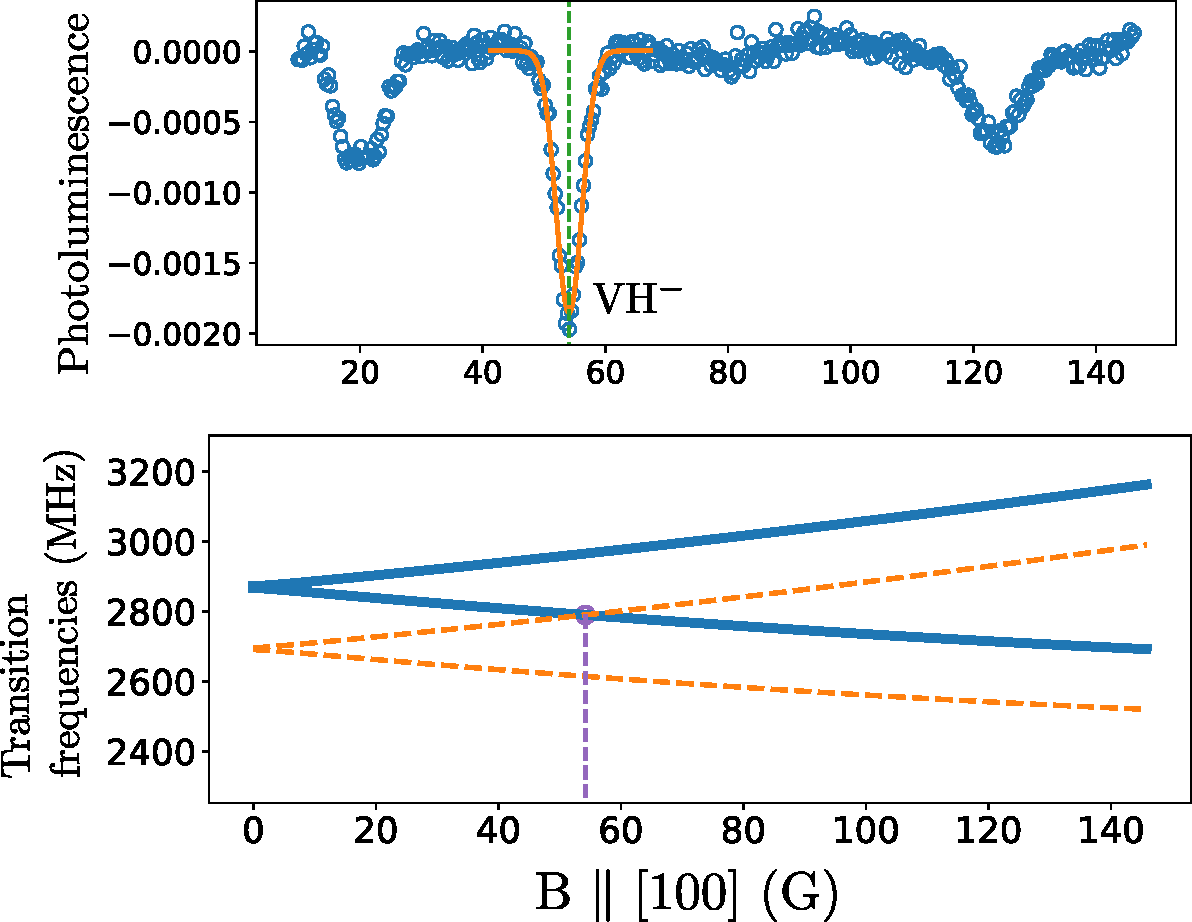
\includegraphics[scale=.48]{soustraction_1}
\end{frame}
\begin{frame}{Cross-relaxation between NV$^-$ and WAR1}
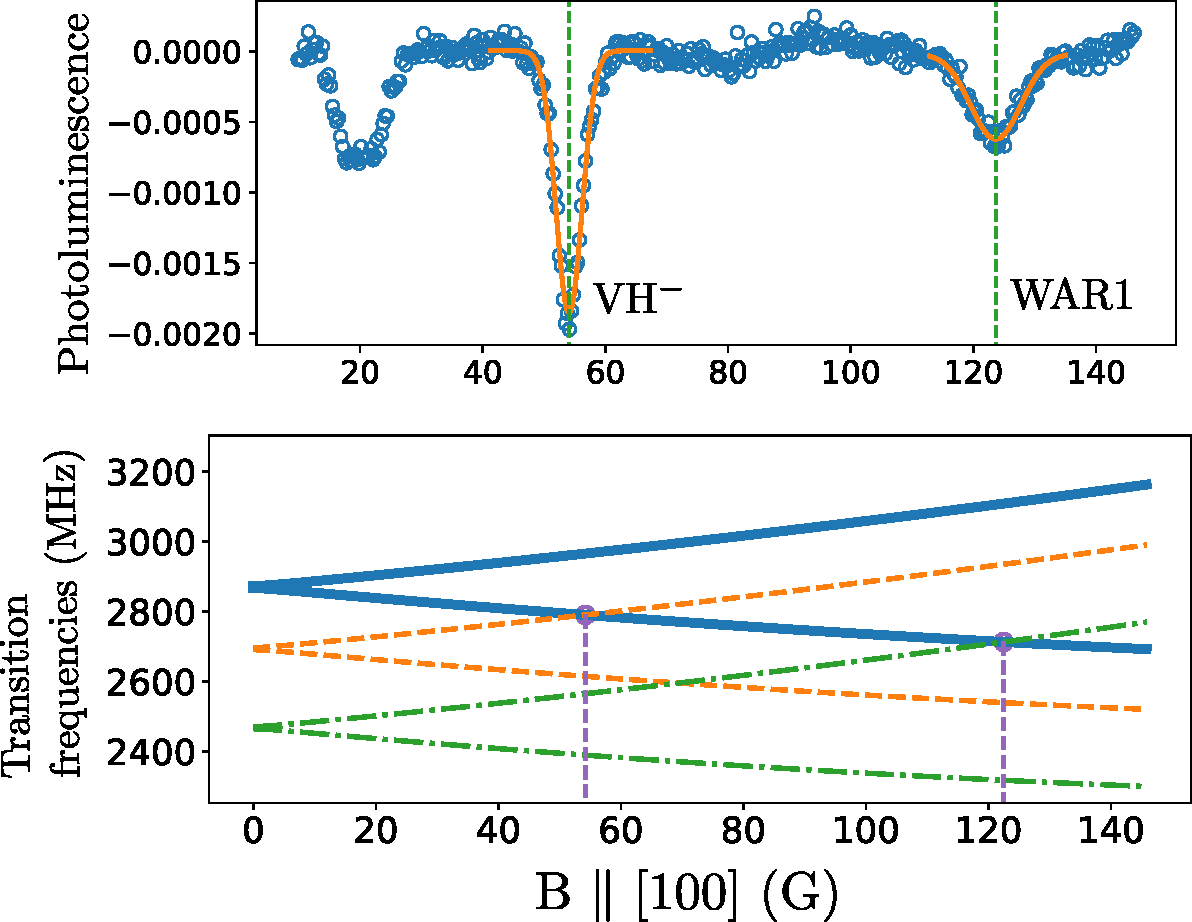
\includegraphics[scale=.48]{soustraction_2}
\end{frame}
\begin{frame}{EPR spectroscopy}
Electron Paramagnetic Resonance : A spectroscopy technique using absorption of a microwave at a given frequency (typically 9.5 GHz) as a function of magnetic field to detect paramagnetic defects.
\bigbreak
VH$^-$\footfullcite{glover_hydrogen_2004} and WAR1 \footfullcite{cruddace2007magnetic} have been observed by EPR spectrocopy in CVD diamonds by Mark Newton's team at the University of Warwick.
\end{frame}
\begin{frame}{Comparison between CR and EPR}
\begin{itemize}
\item CR experiments are much simpler to setup (low $B$, no microwave)
\item NV centers produce a calibration for $B$ $\to$ Better precision on the ZFS measurement
\item Potential for polarization transfer
\bigbreak
\item Requires a high NV concentration and quickly becomes unreadable on non-[100] directions.
\end{itemize}
\end{frame}

\begin{frame}{Cross-relaxation between NV$^-$ and $^{13}$C$-$NV$^-$}
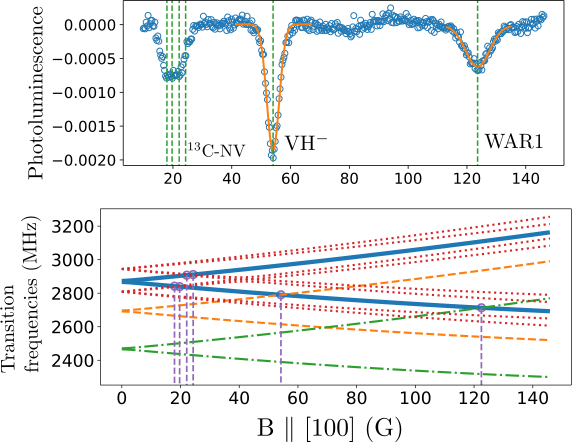
\includegraphics[scale=.48]{soustraction_3}
\end{frame}
\section{Cross-relaxation between NV centers}
\begin{frame}{Outline}
\tableofcontents[currentsection]
\end{frame}
\begin{frame}{Experimental proofs of NV-NV CR}
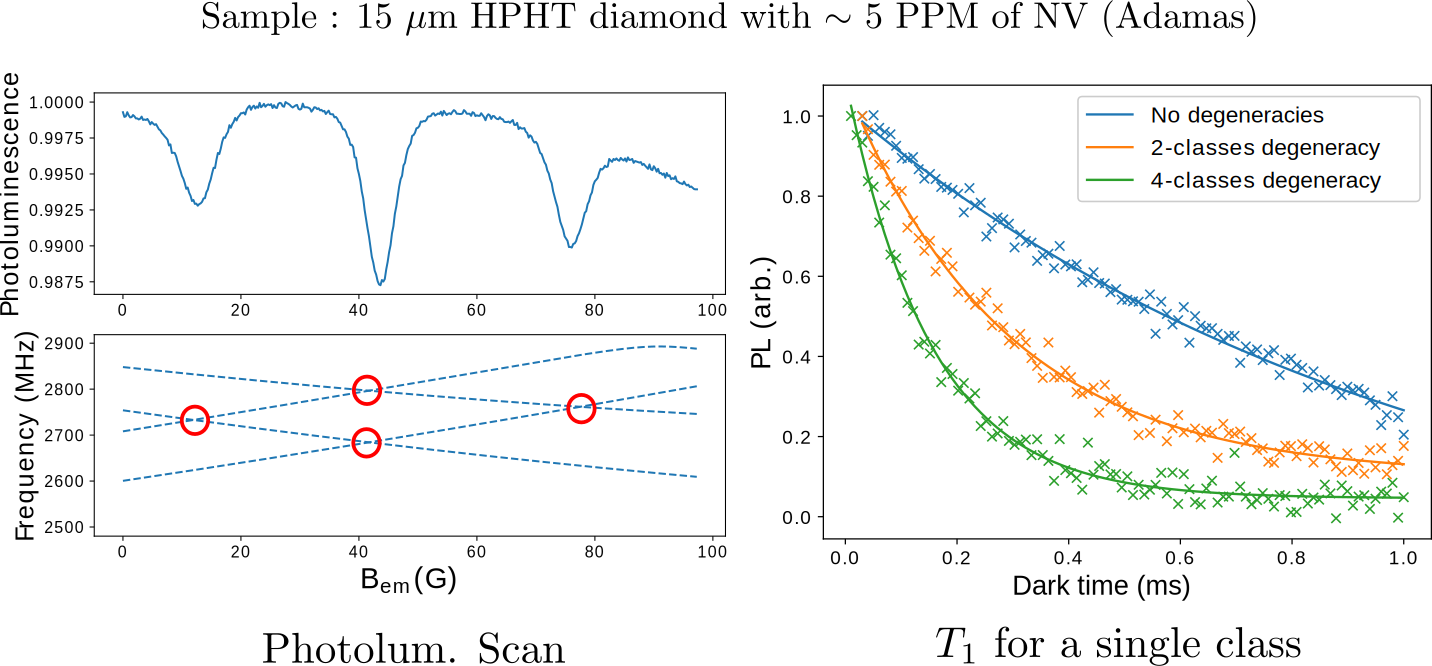
\includegraphics[scale=.28]{NV-NV_0}
\end{frame}
\begin{frame}{Microscopic explanation of the NV-NV CR}
\centering
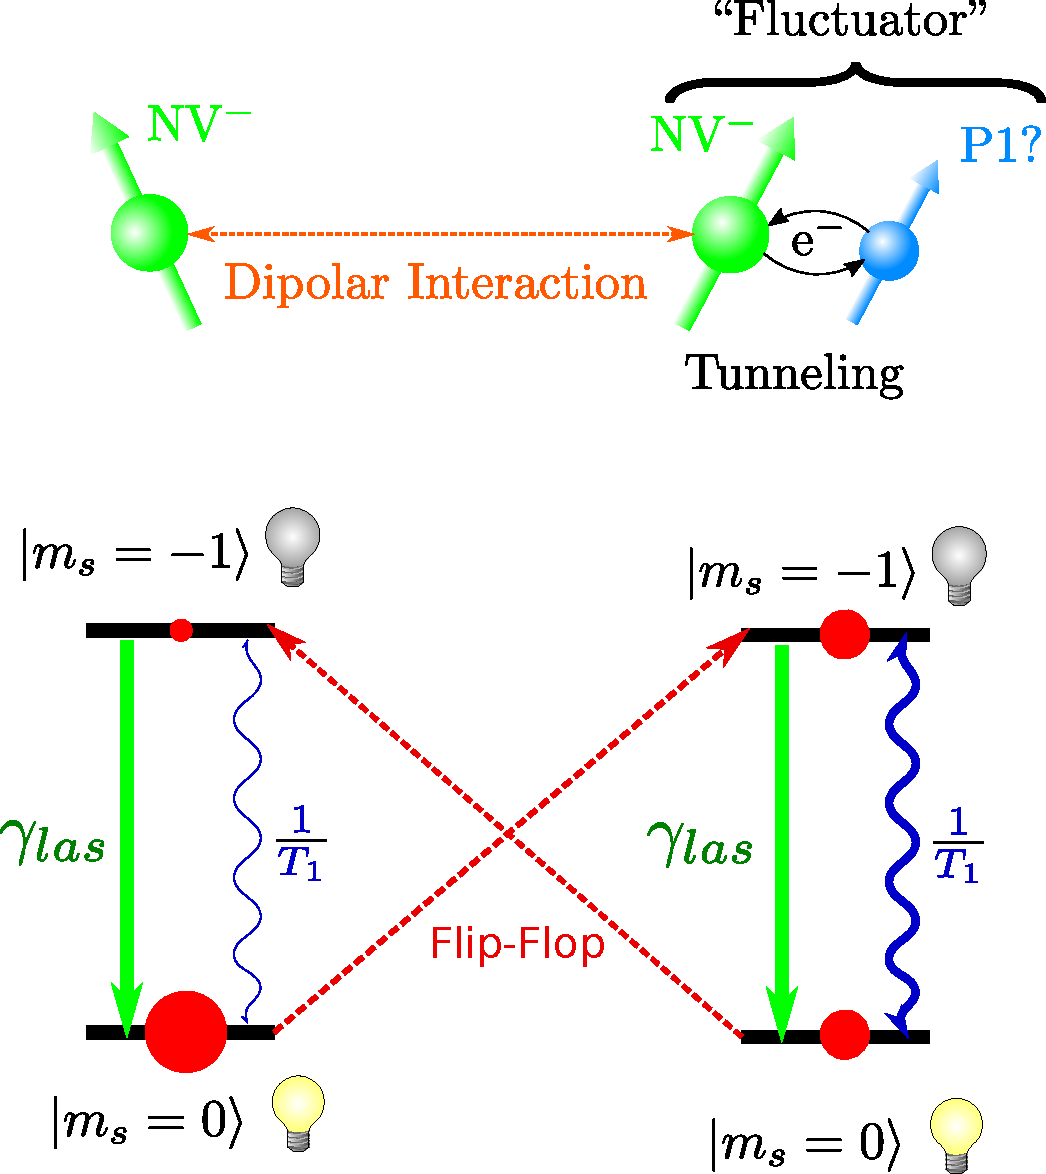
\includegraphics[scale=.35]{NVNV-micro}\footfullcite{choi_depolarization_2017}
\end{frame}
%ajouter la slide avec la carte du coup ?
\section{Torque induced by cross-relaxation on a levitating diamond}
\begin{frame}{Outline}
\tableofcontents[currentsection]
\end{frame}
\begin{frame}{Torque measurement with a levitating diamond}
\centering
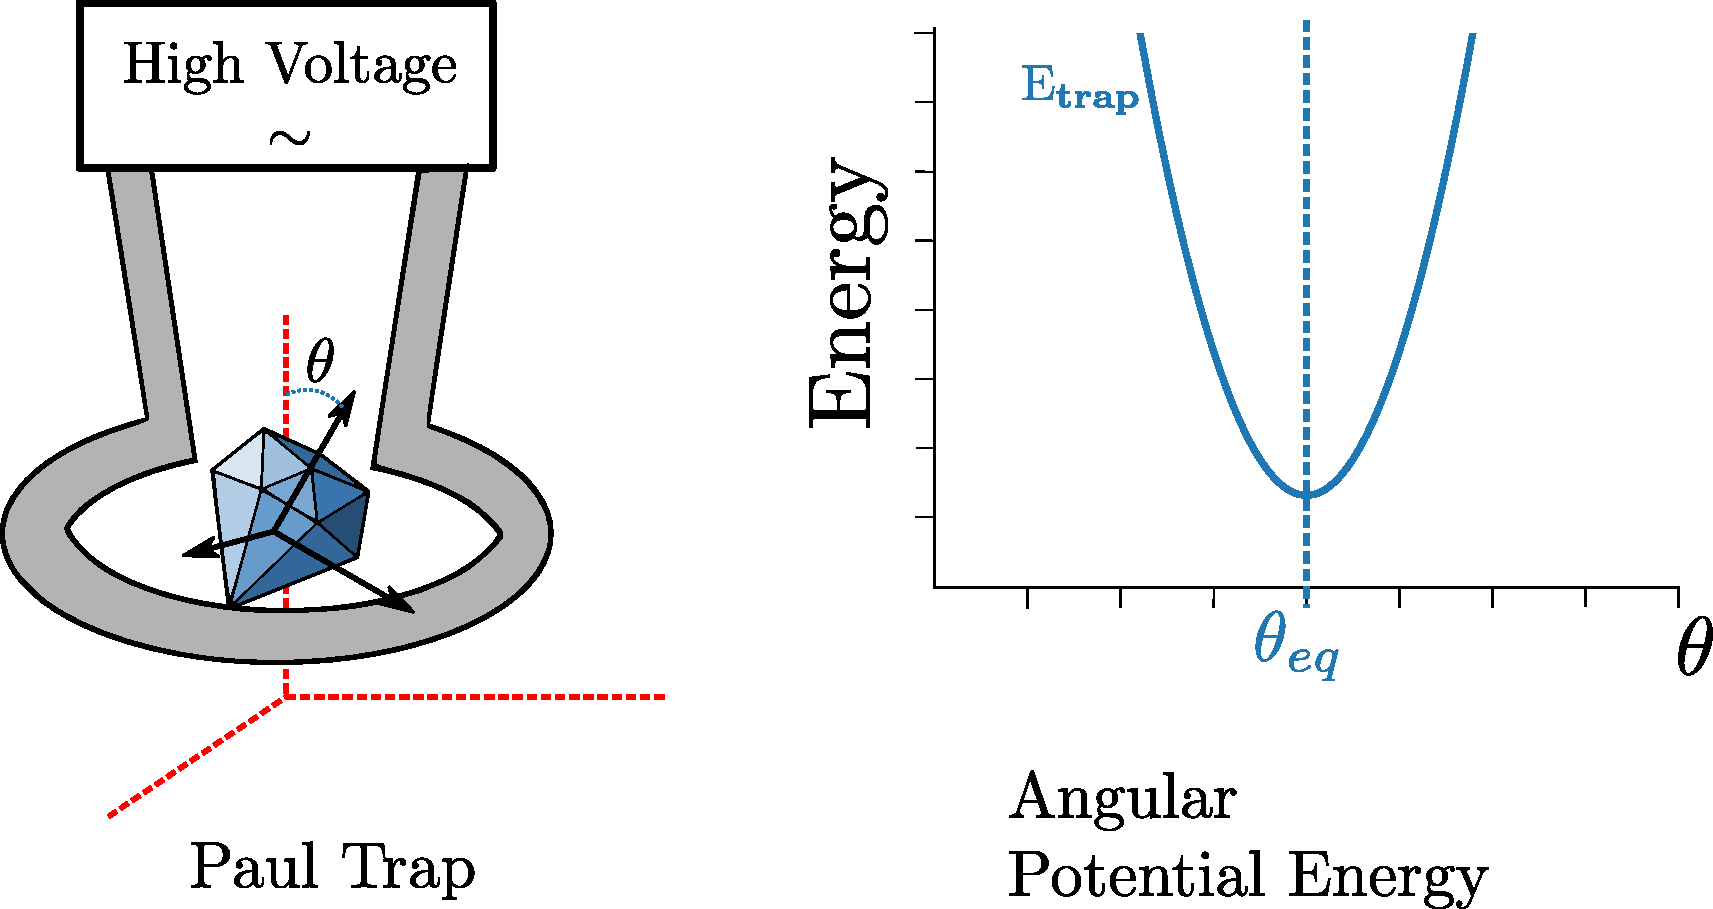
\includegraphics[scale=.3]{Trap_0}%"This trap not only locks the center of mass of the diamond, but it also locks its orientations, because of the anistropy of the trap and of the diamond" "The trap can be roughly modeled by an harmonic potential centered around a particular angle at equilibrium"
\end{frame}
\begin{frame}{Torque potential energy}%"The equivalent of a torque in term of potential energy is a slope"
\centering
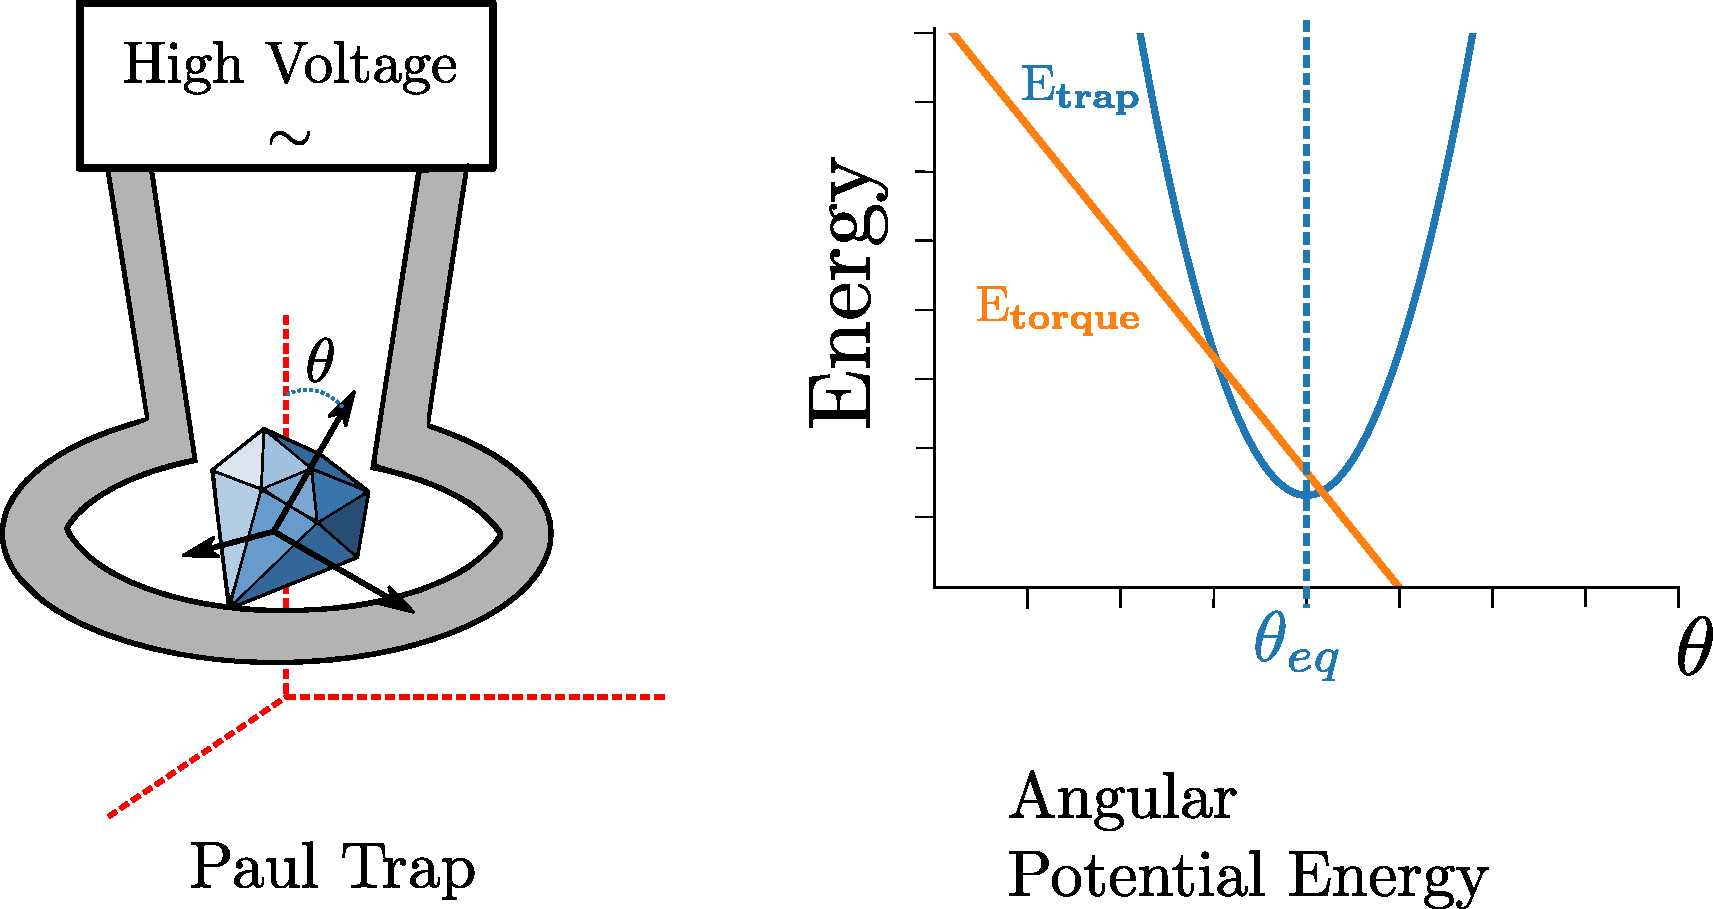
\includegraphics[scale=.3]{Trap_1}
\end{frame}
\begin{frame}{Displacement of equilibrium}
\centering
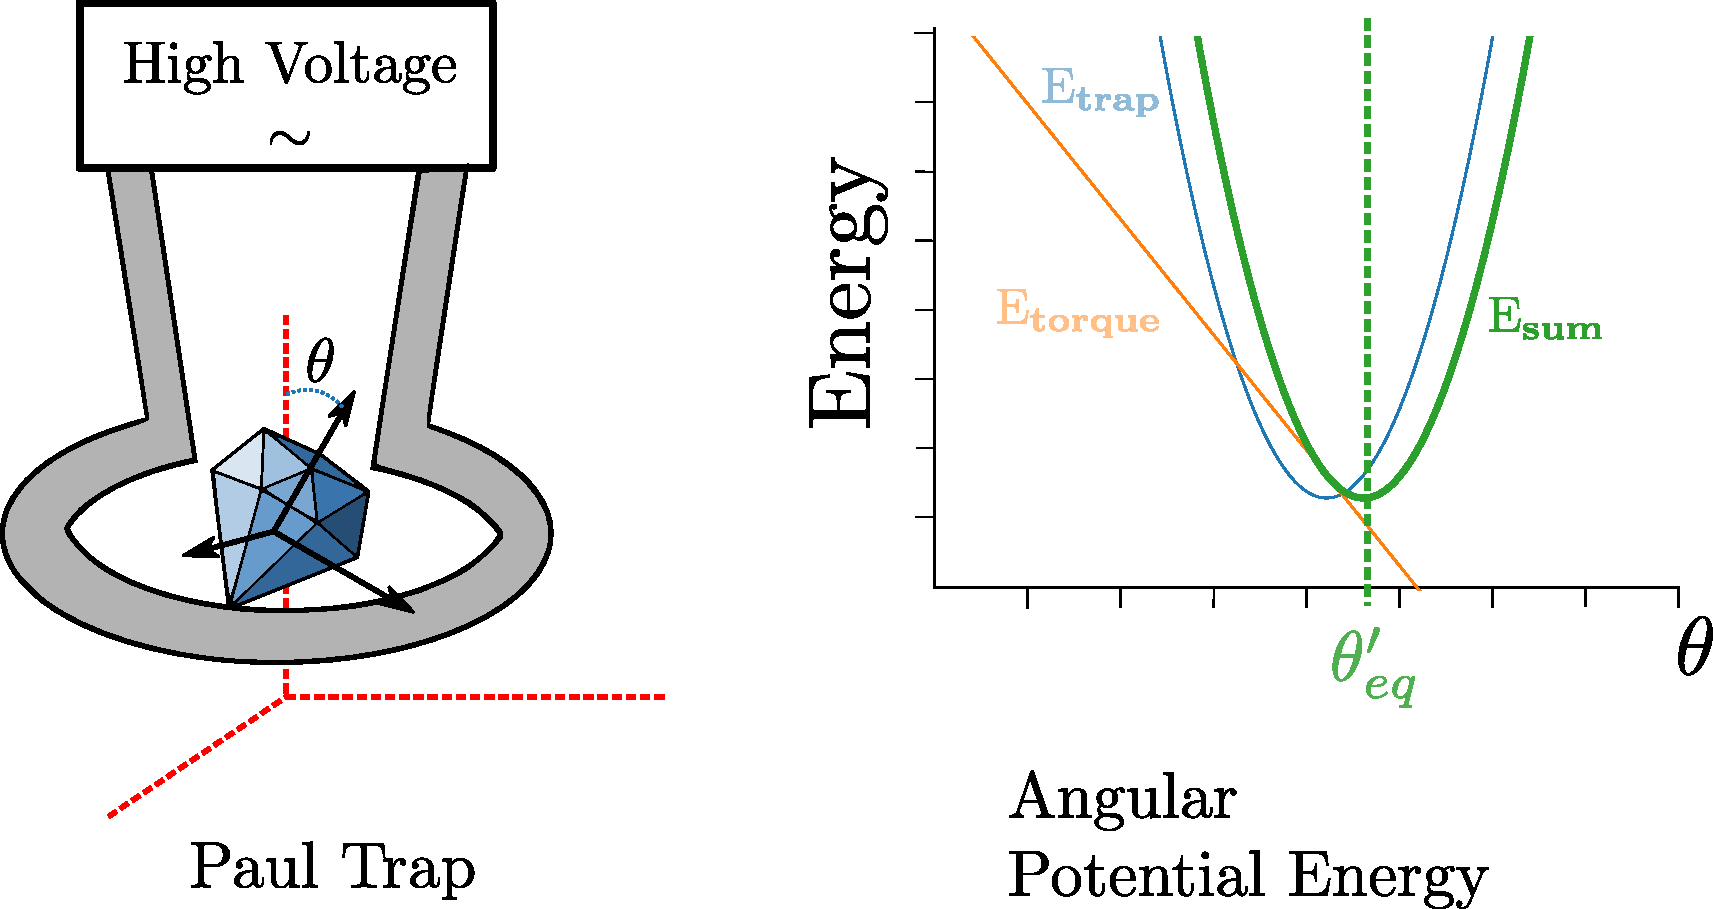
\includegraphics[scale=.3]{Trap_2}
\end{frame}
\begin{frame}{Back-scattered laser detection}
\centering
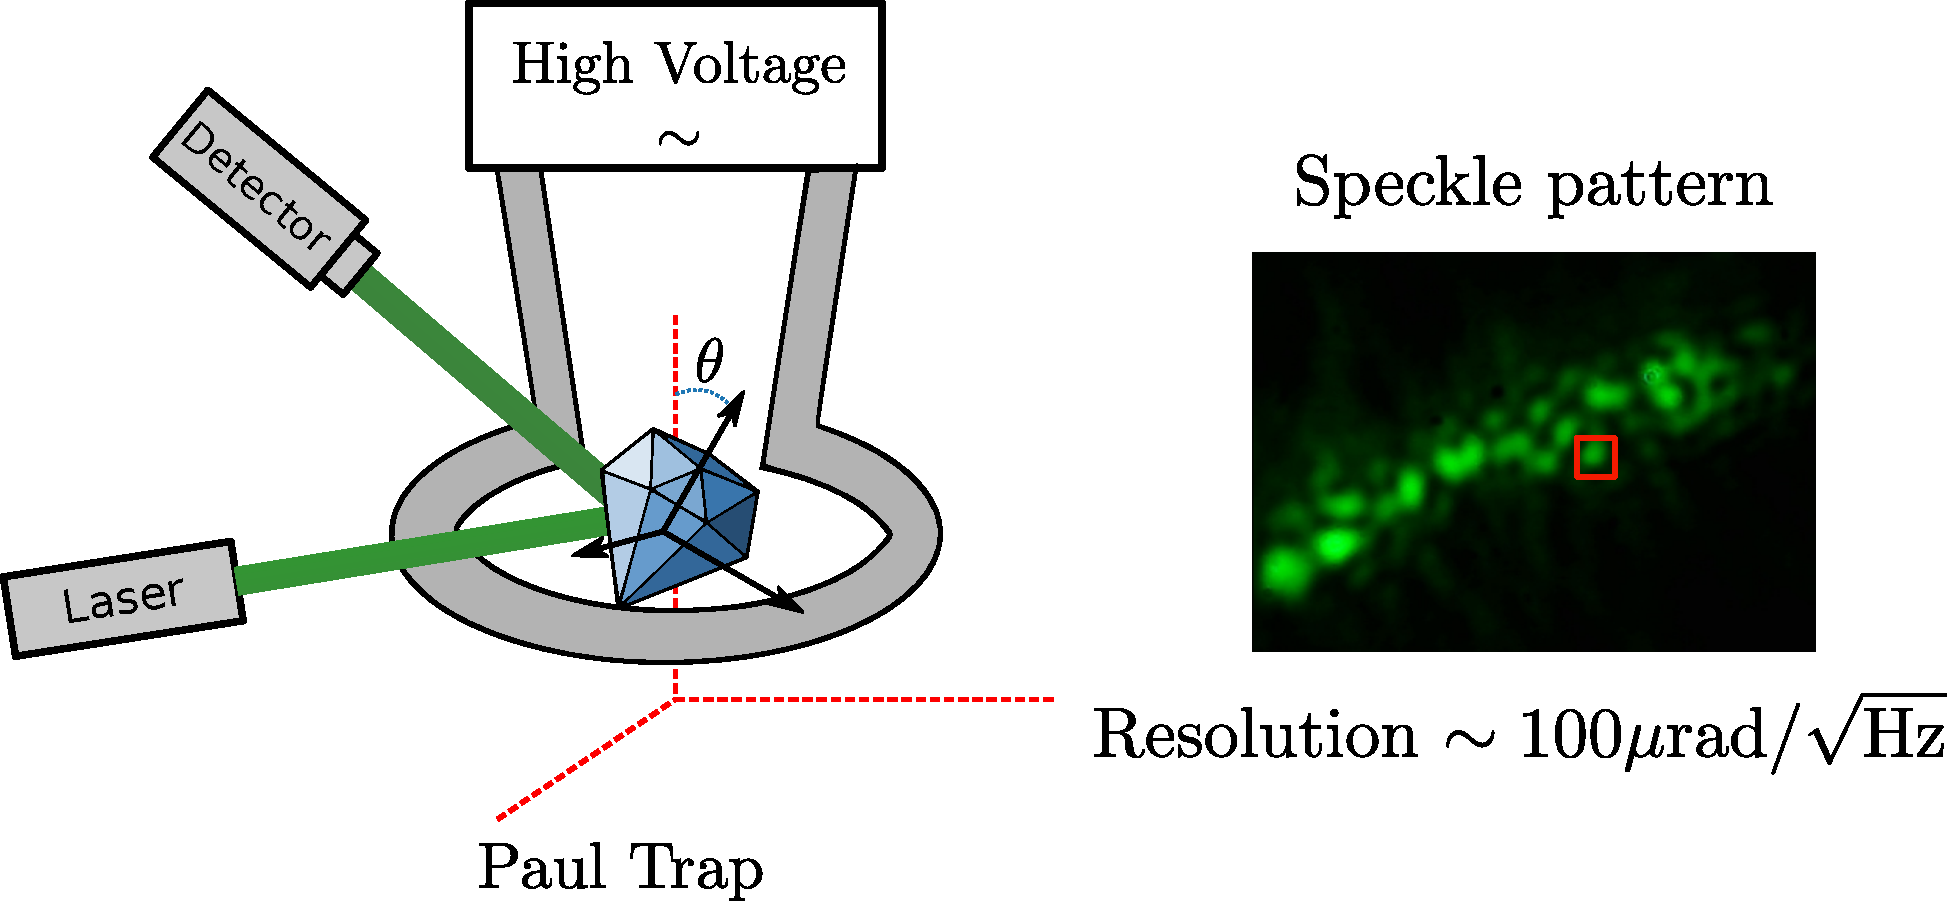
\includegraphics[scale=.3]{Trap_3}%And how do we measure this rotation ? well, since we have to send a laser on the diamond to polarise the NV centers..." "We do not observe a clear reflection of the laser, instead we observe a speckle pattern, which is produced by the many interferences on the rough surface of the diamond" "Whenever the diamond moves, the speckle pattern will either shift or change its shape..."
\end{frame}
\begin{frame}{Torque caused by cross-relaxations}
\centering
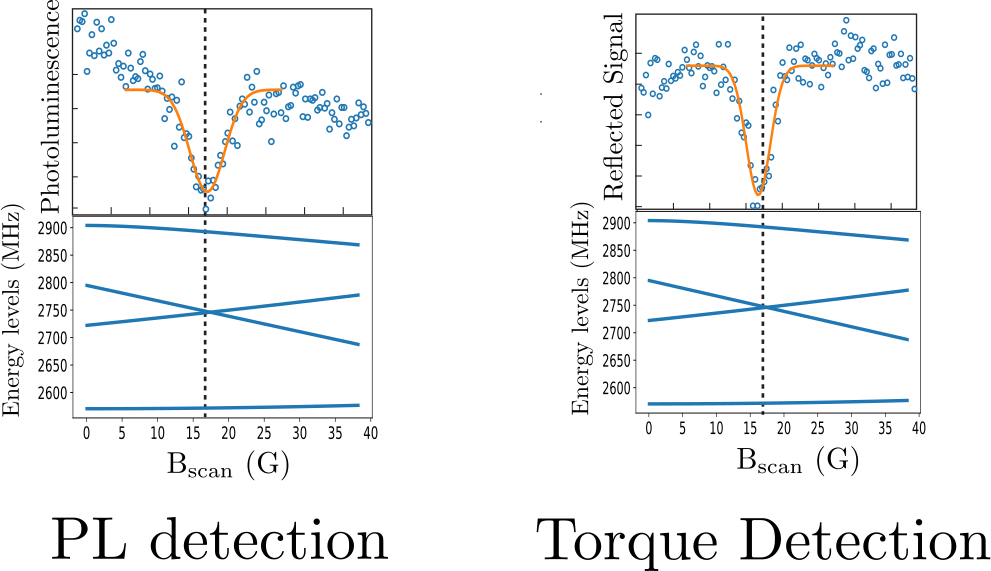
\includegraphics[scale=.4]{CRmeca_121}
\end{frame}
\begin{frame}{Origin of the magnetic torque}
\centering
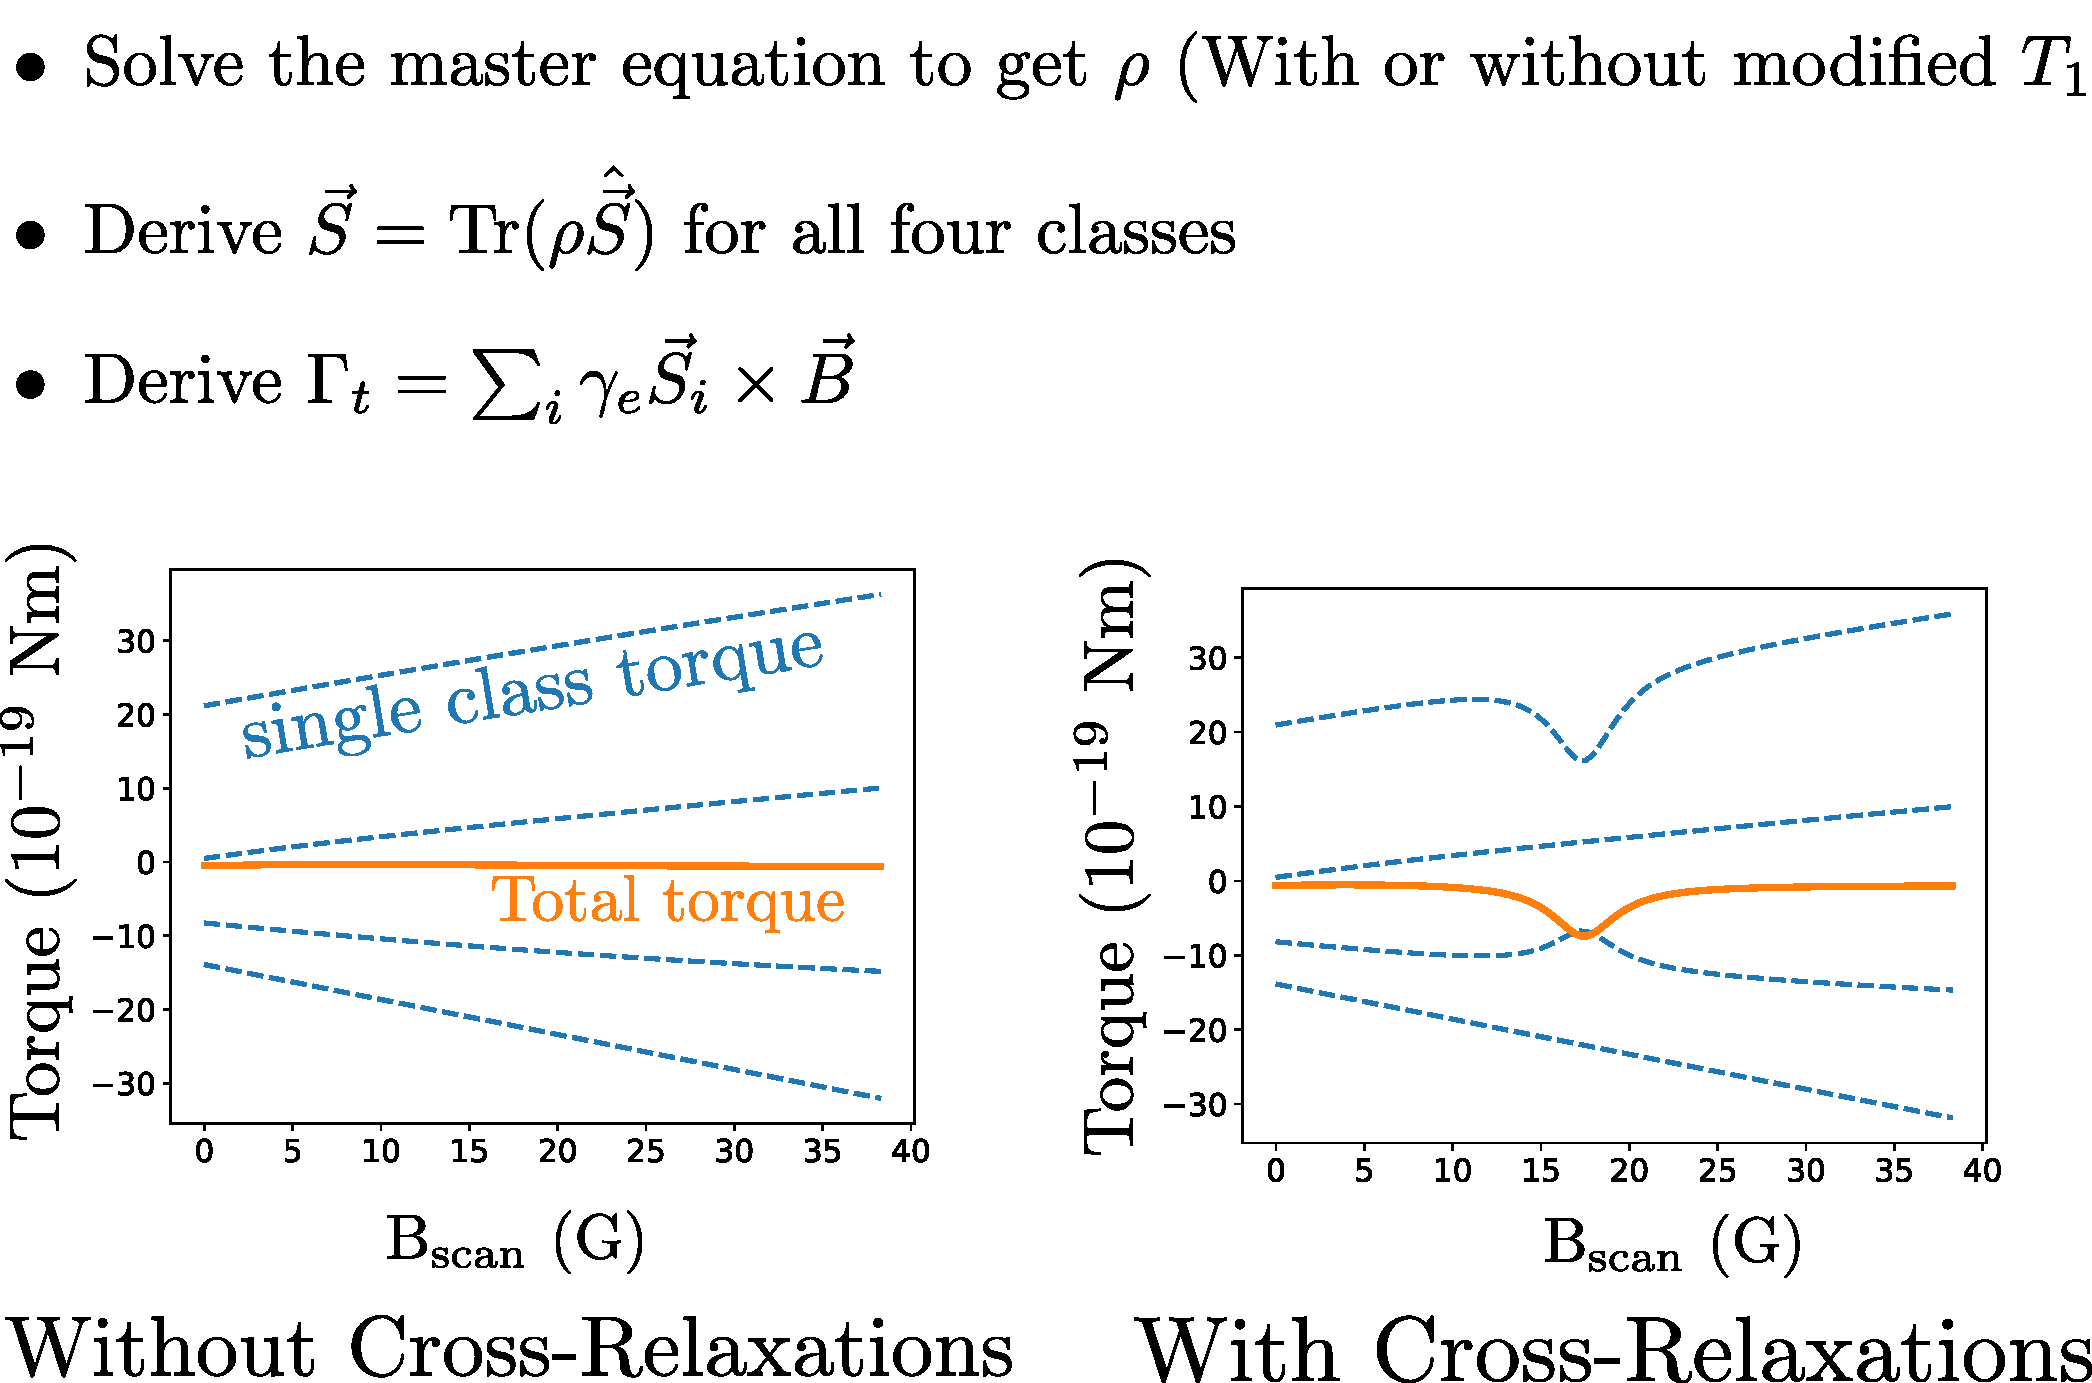
\includegraphics[scale=.3]{Explication_torque}
\end{frame}
\begin{frame}{Torque caused by CR : other configuration}
\centering
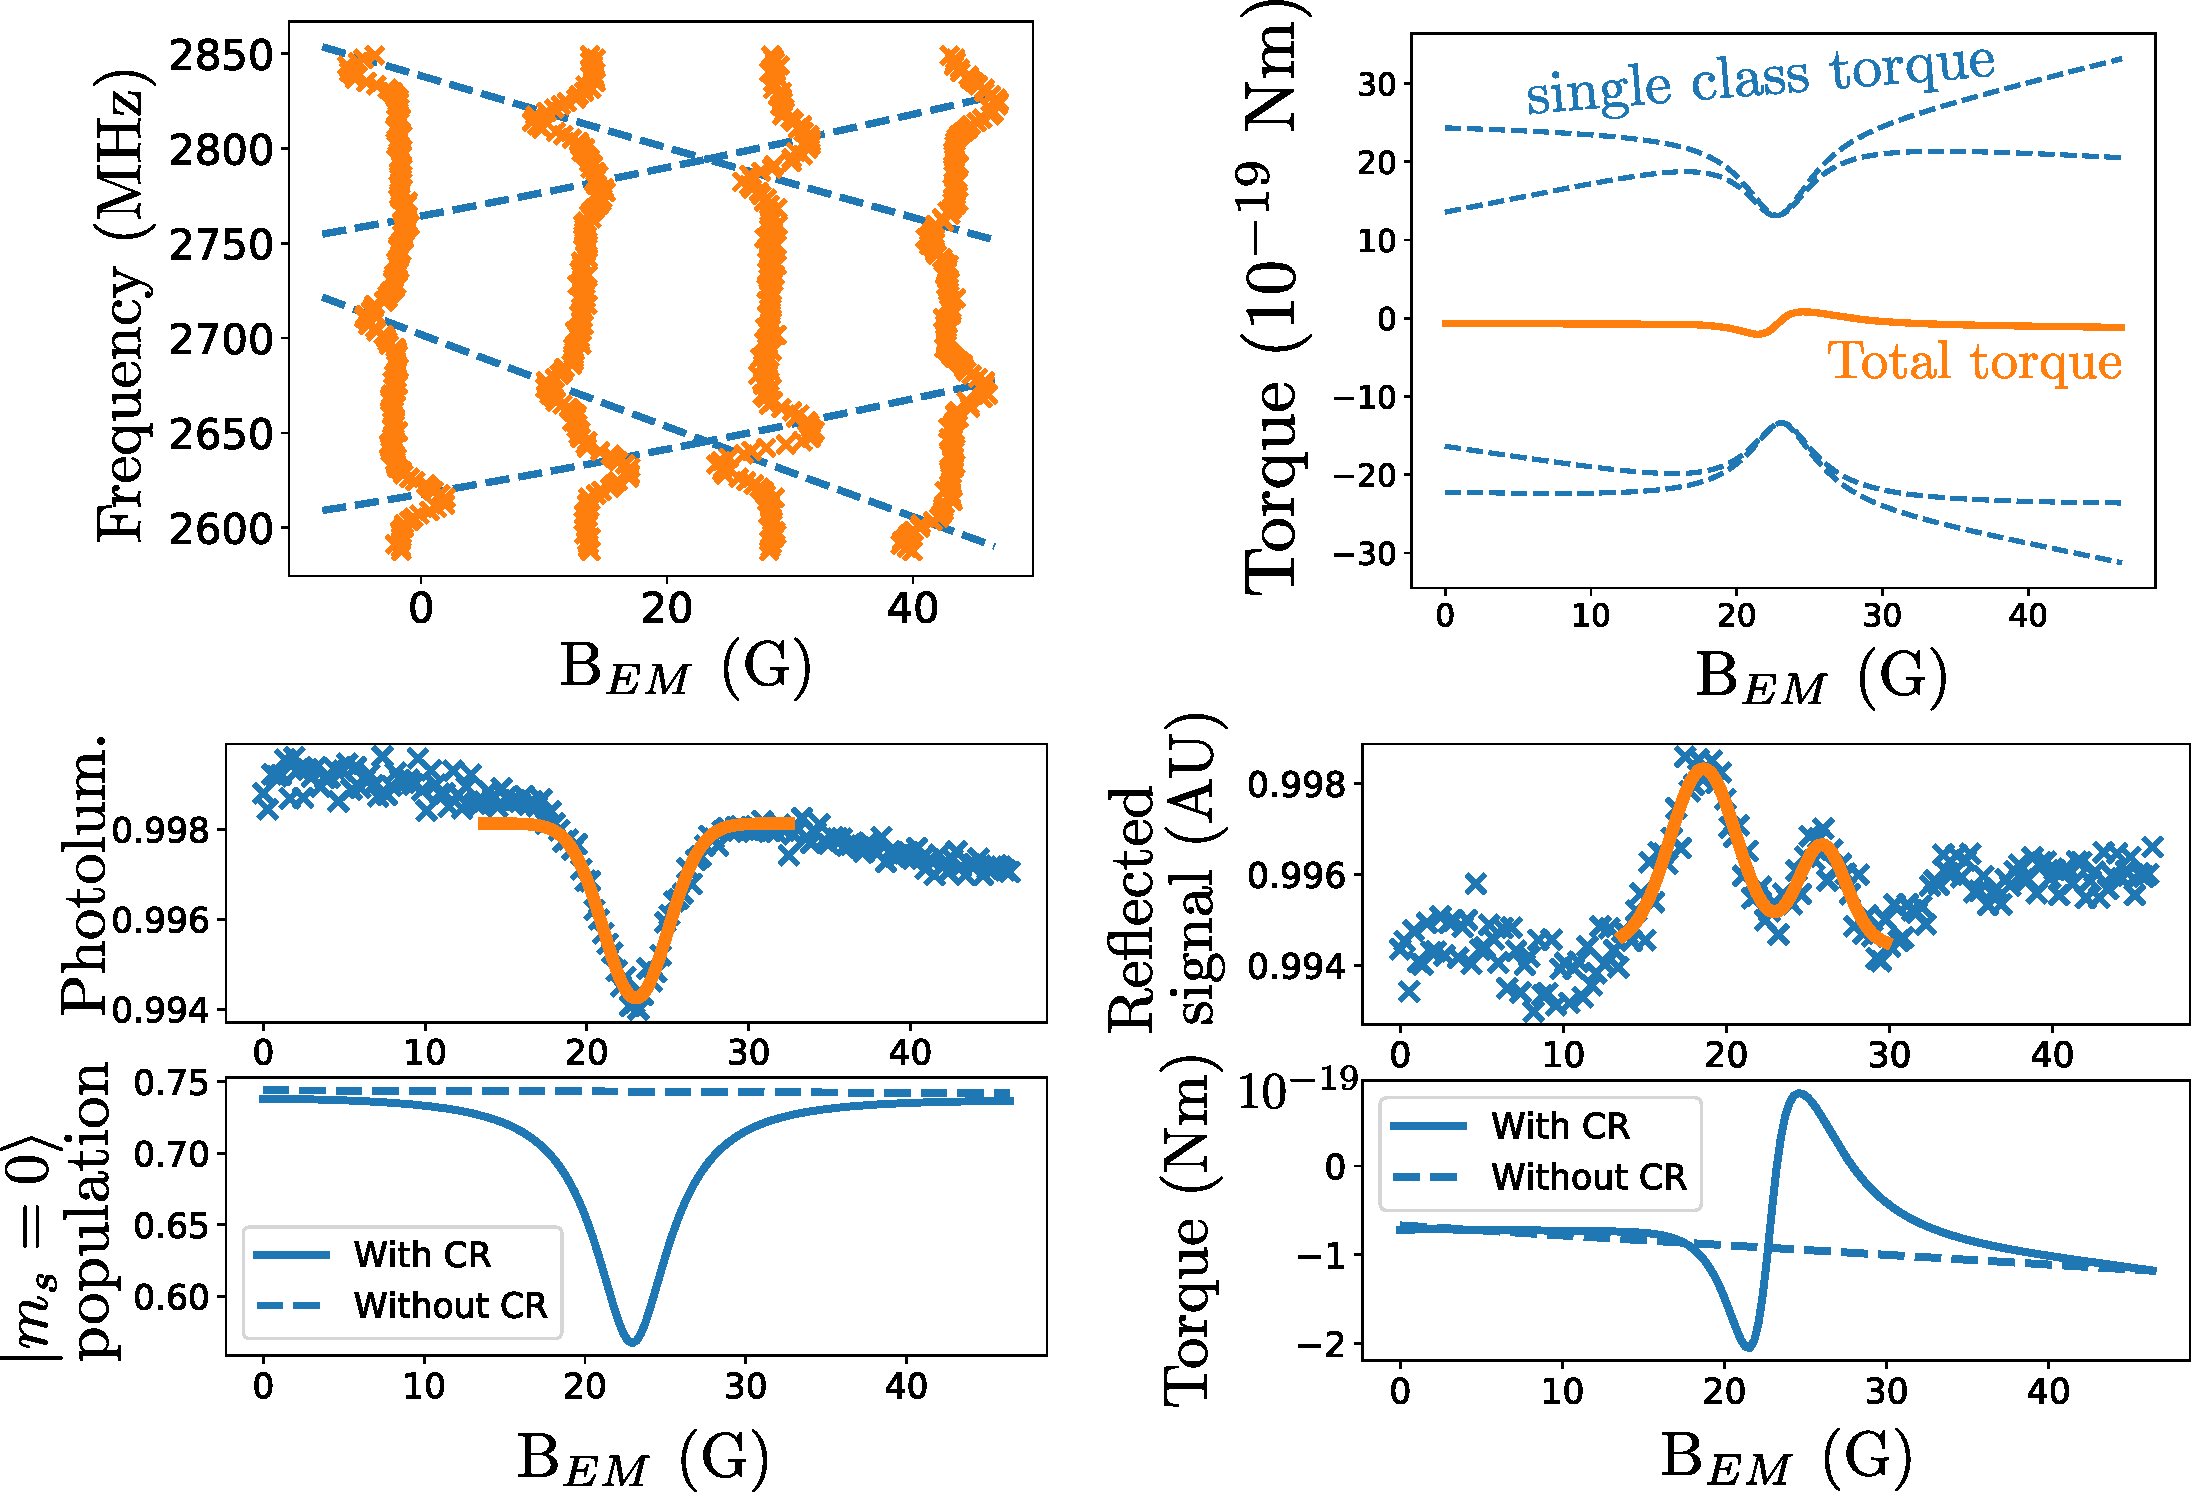
\includegraphics[scale=.28]{CRmeca_22}
\end{frame}
\begin{frame}{Conclusion}
\begin{itemize}
\setlength\itemsep{1em}
\item{Detection of new spin defects in diamond through Cross-Relaxations
\begin{itemize}
\item Potential for hyperpolariaztion of new dark electronic spins
\end{itemize}}
\item{Observations of NV$-$NV Cross-Relaxations}
\item{Mechanical detection of NV$-$NV Cross relaxations :
\begin{itemize}
\item Potential for mechanical detection of new spin species
\item Potential for Resonant Einstein-De-Haas effect 
\end{itemize} }
\end{itemize}
\end{frame}
\end{document}